% The contents of this file is 
% Copyright (c) 2009-  Charles R. Severance, All Righs Reserved

\chapter{데이터베이스와 SQL(Structured Query Language) 사용하기}

\section{데이터베이스가 뭔가요?}
\index{데이터베이스 (database)}

{\bf 데이터베이스(database)}는 데이터를 저장하기 위한 목적으로 조직된 파일이다. 
대부분의 데이터베이스는 키(key)와 값(value)를 매핑한다는 의미에서 딕셔너리처럼 조직되었다.
가장 큰 차이점은 데이터베이스는 디스크(혹은 다른 영구 저장소)에 위치하고 있어서, 프로그램 종료 후에도 정보가 계속 저장된다.
데이터베이스가 영구 저장소에 저장되어서, 컴퓨터 주기억장치(memory) 크기에 제한받는 딕셔너리보다 훨씬 더 많은 정보를 저장할 수 있다.

\index{데이터베이스 (database)!인덱스 (indexes)}

딕셔너리처럼, 데이터베이스 소프트웨어는 엄청난 양의 데이터 조차도 매우 빠르게 삽입하고 접근하도록 설계되었다.
컴퓨터가 특정 항목으로 빠르게 찾아갈 수 있도록 데이터베이스에 {\bf 인덱스(indexes)}를 추가한다.
데이터베이스 소프트웨어는 인덱스를 구축하여 성능을 보장한다.

다양한 목적에 맞춰 서로 다른 많은 데이터베이스 시스템이 개발되어 사용되고 있다. 
Oracle, MySQL, Microsoft SQL Server, PostgreSQL, SQLite이 여기에 포함된다. 
이 책에서는 SQLite를 집중해서 살펴볼 것이다. 
왜냐하면 매우 일반적인 데이터베이스이며 파이썬에 이미 내장되어 있기 때문이다.
응용프로그램 내부에서 데이터베이스 기능을 제공하도록 SQLite가 다른 응용프로그램 내부에 \emph{내장(embedded)}되도록 설계되었다.
예를 들어, 다른 많은 소프트웨어 제품이 그렇듯이, 파이어폭스 브라우져도 SQLite를 사용한다.

\url{http://sqlite.org/}

이번 장에서 기술하는 트위터 스파이더링 응용프로그램처럼 정보과학(Informatics)에서 마주치는 몇몇 데이터 조작 문제에 SQLite가 적합하다.


\section{데이터베이스 개념}
처음 데이터베이스를 볼때 드는 생각은 마치 엑셀같은 다중 시트를 지닌 스프레드쉬트(spreadsheet)같다는 것이다.
데이터베이스에서 주요 데이터 구조물은 {\bf 테이블(tables)}, {\bf 행(rows)}, and {\bf 열(columns)}이 된다. 

\beforefig
\centerline{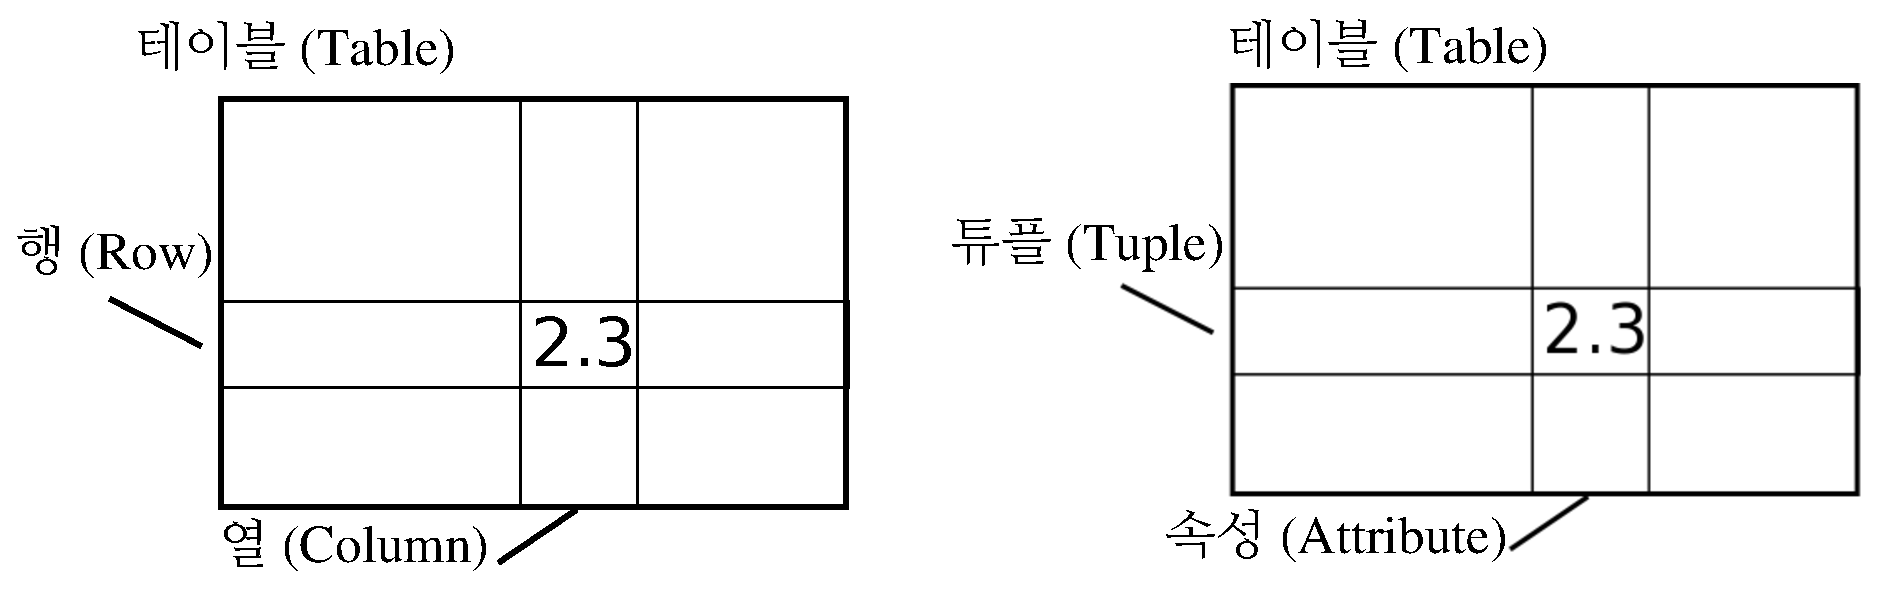
\includegraphics[height=1.50in]{figs2/relational.eps}}
\afterfig

관계형 데이터베이스의 기술적인 면을 설명하면 테이블, 행, 열의 개념은 
{\bf 관계(relation)}, {\bf 튜플(tuple)}, and {\bf 속성(attribute)} 각각 형식적으로 매칭된다.
이번 장에서는 조금 덜 형식 용어를 사용한다.

\section{파이어폭스 애드온 SQLite 매니저}
SQLite 데이터베이스 파일에 있는 데이터를 다루기 위해서 이번장에서 주로 파이썬 사용에 집중을 하지만, 
다음 웹사이트에서 무료로 이용 가능한 {\bf SQLite 데이터베이스 매니저(SQLite Database Manager)}로 불리는 
파이어폭스 애드온(add-on)을 사용해서 좀더 쉽게 많은 작업을 수행할 수 있다.

\url{https://addons.mozilla.org/en-us/firefox/addon/sqlite-manager/}

브라우져를 사용해서 쉽게 테이블을 생성하고, 데이터를 삽입, 편집하고 데이터베이스 데이터에 대해 간단한 SQL 질의를 실행할 수 있다.

이러한 점에서 데이터베이스 매니저는 텍스트 파일을 작업할 때 사용하는 텍스트 편집기와 유사하다.
텍스트 파일에 하나 혹은 몇개 작업만 수행하고자 하면, 텍스트 편집기에서 파일을 열어 필요한 수정작업을 하고 닫으면 된다.
텍스트 파일에 작업할 사항이 많은 경우는 종종 간단한 파이썬 프로그램을 작성하여 수행한다.
데이터베이스로 작업할 때도 동일한 패턴이 발견된다. 
간단한 작업은 데이터베이스 매니저를 통해서 수행하고,
좀더 복잡한 작업은 파이썬으로 수행하는 것이 더 편리하다.


\section{데이터베이스 테이블 생성하기}

데이터베이스는 파이썬 리스트 혹은 딕셔너리보다 좀더 명확히 정의된 구조를 요구한다.\footnote{
실질적으로 SQLite는 열에 저장되는 데이터 형식에 대해서 좀더 많은 유연성을 부여하지만,
이번 장에서는 데이터 형식을 엄격하게 적용해서 MySQL 같은 다른 관계형 데이터베이스 시스템에도 동일한 개념이 적용되게 한다.}.  

데이터베이스에 {\bf 테이블(table)}을 생성할 때, {\bf 열(column)}의 명칭과 각 {\bf 열(column)}에 저장하는 테이터 형식을 사전에 정의해야 한다. 
데이터베이스 소프트웨어가 각 열의 데이터 형식을 인식하게 되면, 데이터 형식에 따라 데이터를 저장하고 찾아오는 방법을 가장 효율적인 방식을 선택할 수 있다.

다음 url에서 SQLite에서 지원되는 다양한 데이터 형식을 살펴볼 수 있다.

\url{http://www.sqlite.org/datatypes.html}

처음에는 데이터 구조를 사전에 정의하는 것이 불편하게 보이지만, 대용량의 데이터가 데이터베이스에 포함되더라도 데이터의 빠른 접근을 보장하는 잇점이 있다.

데이터베이스 파일과 데이터베이스에 두개의 열을 가진 {\tt Tracks} 이름의 테이블을 생성하는 코드는 다음과 같다.

\index{sqlite3 module}
\index{module!sqlite3}
\beforeverb
\begin{verbatim}
import sqlite3

conn = sqlite3.connect('music.sqlite3')
cur = conn.cursor()

cur.execute('DROP TABLE IF EXISTS Tracks ')
cur.execute('CREATE TABLE Tracks (title TEXT, plays INTEGER)')

conn.close()
\end{verbatim}
\afterverb
%

\index{연결 함수 (connect function)}
\index{함수 (function)!연결 (connect)}
\index{커서 함수 (cursor function)}
\index{함수 (function)!커서 (cursor)}

{\tt 연결 (connect)} 연산은 현재 디렉토리 {\tt music.sqlite3} 파일에 저장된 데이터베이스에 ''연결(connection)''한다.
파일이 존재하지 않으면, 자동 생성된다. 
''연결(connection)''이라고 부르는 이유는 때때로 데이터베이스가 응용프로그램이 실행되는 서버로부터
분리된 ''데이터베이스 서버(database server)''에 저장되기 때문이다.
지금 간단한 예제 파일의 경우에 데이터베이스가 로컬 파일 형태로 파이썬 코드 마찬가지로 동일한 디렉토리에 있다.

파일을 다루는 파일 핸들(file handle)처럼 데이터베이스에 저장된 파일에 연산을 수행하기 위해서 {\bf 커서(cursor)}를 사용한다.
{\tt cursor()}를 호출하는 것은 개념적으로 텍스트 파일을 다룰 때 {\tt open()}을 호출하는 것과 개념적으로 매우 유사하다.

\beforefig
\centerline{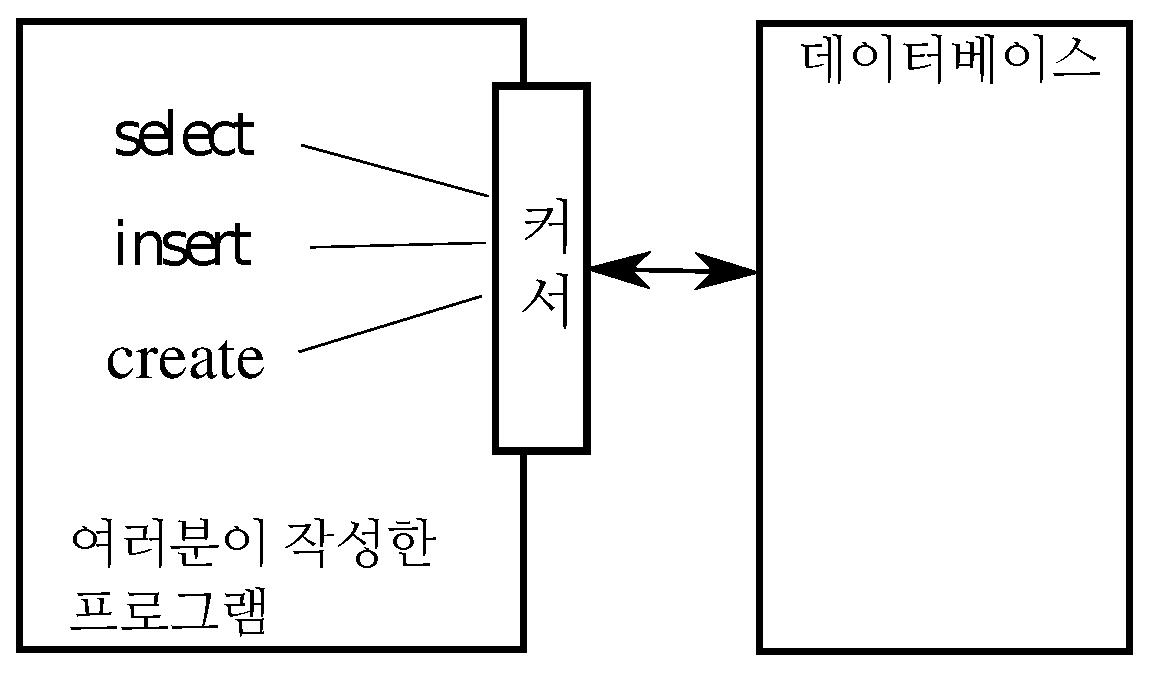
\includegraphics[height=1.50in]{figs2/cursor.eps}}
\afterfig

커서가 생성되면, {\tt execute()} 메쏘드를 사용하여 데이터베이스 콘텐츠에 명령어 실행을 할 수 있다.

데이터베이스 명령어는 특별한 언어로 표현된다.
단일 데이터베이스 언어를 학습하도록 서로 다른 많은 데이터베이스 업체 사이에서 표준화되었다.

데이터베이스 언어를 {\bf SQL(Structured Query Language 구조적 질의 언어)}로 부른다.

\url{http://en.wikipedia.org/wiki/SQL}

상기 예제에서, 데이터베이스에 두개의 SQL 명령어를 실행했다. 
관습적으로 데이터베이스 키워드는 대문자로 표기한다.
테이블명이나 열의 명칭처럼 사용자가 추가한 명령어 부분은 소문자로 표기한다.

첫 SQL 명령어는 만약 존재한다면 데이터베이스에서 {\tt Tracks} 테이블을 삭제한다.
동일한 프로그램을 실행해서 오류 없이 반복적으로 {\tt Tracks} 테이블을 생성하도록하는 패턴이다.
{\tt DROP TABLE} 명령어는 데이터베이스 테이블 및 테이블 콘텐츠 전부를 삭제하니 주의한다. (즉, ''실행취소(undo)''가 없다.)

\beforeverb
\begin{verbatim}
cur.execute('DROP TABLE IF EXISTS Tracks ')
\end{verbatim}
\afterverb
%

두번째 명령어는 {\tt title} 문자형 열과 {\tt plays} 정수형 열을 가진 {\tt Tracks}으로 명명된 테이블을 생성한다.

\beforeverb
\begin{verbatim}
cur.execute('CREATE TABLE Tracks (title TEXT, plays INTEGER)')
\end{verbatim}
\afterverb
%

이제 {\tt Tracks}으로 명명된 테이블을 생성했으니, SQL {\tt INSERT} 연산을 통해 테이블에 데이터를 넣을 수 있다.
다시 한번, 데이터베이스에 연결하여 {\tt 커서(cursor)}를 얻어 작업을 시작한다. 
그리고 나서 커서를 사용해서 SQL 명령어를 수행한다.

SQL {\tt INSERT} 명령어는 어느 테이블을 사용할지 특정한다.
그리고 나서 {\tt (title, plays) } 포함할 필드 목록과 테이블 새로운 행에 저장될 {\tt VALUES} 나열해서 신규 행을 정의를 마친다.
실제 값이 {\tt execute()} 호출의 두번째 매개변수로 튜플{\tt ( 'My Way', 15 ) }로 넘겨는 것을 표기하기 위해서 값을 물음표 {\tt (?, ?)}로 명기한다.

\beforeverb
\begin{verbatim}
import sqlite3

conn = sqlite3.connect('music.sqlite3')
cur = conn.cursor()

cur.execute('INSERT INTO Tracks (title, plays) VALUES ( ?, ? )', 
    ( 'Thunderstruck', 20 ) )
cur.execute('INSERT INTO Tracks (title, plays) VALUES ( ?, ? )', 
    ( 'My Way', 15 ) )
conn.commit()

print 'Tracks:'
cur.execute('SELECT title, plays FROM Tracks')
for row in cur :
   print row

cur.execute('DELETE FROM Tracks WHERE plays < 100')
conn.commit()

cur.close()
\end{verbatim}
\afterverb
%

먼저 테이블에 두개 열을 {\tt 삽입(INSERT)}하고 {\tt commit()} 명령어를 사용하여 데이터가 데이터베이스에 저장되도록 했다.

\beforefig
\centerline{\includegraphics[height=1.00in]{figs2/tracks.eps}}
\afterfig

그리고 나서, {\tt SELECT} 명령어를 사용하여 테이블에 방금 전에 삽입한 행을 불러왔다.
{\tt SELECT} 명령어에서 데이터를 어느 열{\tt (title, plays)}에서, 어느 테이블{\tt Tracks}에서 을 가져올지 명세한다.
{\tt SELECT} 명령문을 수행한 후에, 커서는 {\tt for}문 반복을 수행하는 것과 같다.
효율성을 위해서, 커서가 {\tt SELECT} 명령문을 수행할 때 데이터베이스에서 모든 데이터를 읽지 않는다. 
대신에 {\tt for}문에서 행을 반복해서 가져하듯이 요청시에만 데이터를 읽어온다.

프로그램 실행결과는 다음과 같다.

\beforeverb
\begin{verbatim}
Tracks:
(u'Thunderstruck', 20)
(u'My Way', 15)
\end{verbatim}
\afterverb
%
\index{유니코드 (Unicode)}

{\tt for} 루프가 행을 두개를 읽어왔다. 
각각의 행은 {\tt title}로 첫번째 값을,{\tt plays}로 두번째 값을 갖는 파이썬 튜플이다. 
title 문자열이 u'로 시작한다고 걱정하지 마라.
해당 문자열은 라틴 문자가 아닌 다국어를 저장할 수 있는 {\bf 유니코드(Unicode)} 문자열을 나타내는 것이다.

프로그램 마지막에 SQL 명령어를 실행 사용해서 방금전에 생성한 행을 모두 {\tt 삭제(DELETE)}했기 때문에 
프로그램을 반복해서 실행할 수 있다. 
{\tt 삭제(DELETE)} 명령어는 {\tt WHERE} 문을 사용하여 선택 조건을 표현할 수 있다.
따라서 명령문에 조건을 충족하는 행에만 명령문을 적용한다.
이번 예제에서 기준이 모든 행에 적용되어 테이블에 아무 것도 없게 된다.
따라서 프로그램을 반복적으로 실행할 수 있다.
{\tt 삭제(DELETE)}를 실행한 후에 {\tt commit()}을 호출하여 데이터베이스에서 데이터를 완전히 제거했다.

\section{SQL(Structured Query Language) 요약}

지금까지, 파이썬 예제를 통해서 SQL(Structured Query Language)을 사용했고, SQL 명령어에 대한 기본을 다루었다.
이번 장에서는 SQL 언어를 보고 SQL 구문 개요를 살펴본다.

대단히 많은 데이터베이스 업체가 존재하기 때문에 호환성의 문제로 SQL(Structured Query Language)이 표준화되었다.
그래서, 여러 업체가 개발한  데이터베이스 시스템 사이에 호환하는 방식으로 커뮤니케이션 가능하다.

관계형 데이터베이스는 테이블, 행과 열로 구성된다. 
열(column)은 일반적으로 텍스트, 숫자, 혹은 날짜 자료형을 갖는다.
테이블을 생성할 때, 열의 명칭과 자료형을 지정한다.

\beforeverb
\begin{verbatim}
CREATE TABLE Tracks (title TEXT, plays INTEGER)
\end{verbatim}
\afterverb
%

테이블에 행을 삽입하기 위해서 SQL {\tt INSERT} 명령어를 사용한다.

\beforeverb
\begin{verbatim}
INSERT INTO Tracks (title, plays) VALUES ('My Way', 15)
\end{verbatim}
\afterverb
%

{\tt INSERT} 문장은 테이블 이름을 명기한다.
그리고 나서 새로운 행에 놓고자 하는 열/필드 리스트를 명시한다.
그리고 나서 키워드 {\tt VALUES}와 각 필드 별로 해당하는 값을 넣는다.

SQL {\tt SELECT} 명령어는 데이터베이스에서 행과 열을 가져오기 위해 사용된다.
{\tt SELECT} 명령문은 가져오고자 하는 행과 {\tt WHERE}절을 사용하여 어느 행을 가져올지 지정한다.
선택 사항으로 {\tt ORDER BY} 절을 이용하여 반환되는 행을 정렬할 수도 있다.

\beforeverb
\begin{verbatim}
SELECT * FROM Tracks WHERE title = 'My Way'
\end{verbatim}
\afterverb
%

\verb"*" 을 사용하여 {\tt WHERE} 절에 매칭되는 각 행의 모든 열을 데이터베이스에서 가져온다.

주목할 점은 파이썬과 달리 SQL {\tt WHERE} 절은 등식을 시험하기 위해서 두개의 등치 기호 대신에 단일 등치 기호를 사용한다.
{\tt WHERE}에서 인정되는 다른 논리 연산자는 
\verb"<",
\verb">",
\verb"<=",
\verb">=",
\verb"!=" 이고, 논리 표현식을 생성하는데 {\tt AND}, {\tt OR}, 괄호를 사용한다.

다음과 같이 반환되는 행이 필드값 중 하나에 따라 정렬할 수도 있다.

\beforeverb
\begin{verbatim}
SELECT title,plays FROM Tracks ORDER BY title
\end{verbatim}
\afterverb
%

행을 제거하기 위해서, SQL {\tt DELETE} 문장에 {\tt WHERE} 절이 필요하다.
{\tt WHERE} 절이 어느 행을 삭제할지 결정한다.

\beforeverb
\begin{verbatim}
DELETE FROM Tracks WHERE title = 'My Way'
\end{verbatim}
\afterverb
%

다음과 같이 SQL {\tt UPDATE} 문장을 사용해서 테이블에 하나 이상의 행 내에 있는 하나 이상의 열을 {\tt 갱신(UPDATE)}할 수 있다.

\beforeverb
\begin{verbatim}
UPDATE Tracks SET plays = 16 WHERE title = 'My Way'
\end{verbatim}
\afterverb
%

{\tt UPDATE} 문장은 먼저 테이블을 명시한다.
그리고 나서, {\tt SET} 키워드 다음에 변경할 필드 리스트 와 값을 명시한다.
그리고 선택사항으로 갱신될 행을 {\tt WHERE}절에 지정한다. 
단일 {\tt UPDATE} 문장은 {\tt WHERE}절에서 매칭되는 모든 행을 갱신한다. 
혹은 만약 {\tt WHERE}절이 지정되지 않으면,테이블 모든 행에 대해서 {\tt 갱신(UPDATE)}을 한다.

네가지 기본 SQL 명령문(INSERT, SELECT, UPDATE, DELETE)은 데이터를 생성하고 유지 관리하는데 필요한 기본적인 4가지 작업을 가능케 한다.

\section{데이터베이스를 사용한 트위터 스파이더링(Spidering)}

이번장에서 트위커 계정을 조사하고 데이터베이스를 생성하는 간단한 스파이더링 프로그램을 작성합니다.
\emph{주의: 프로그램을 실행할 때 매우 주의하세요. 여러분의 트위터 계정 접속이 차단될 정도로 너무 많은 데이터를 가져오거나 
장시간 프로그램을 실행하지 마세요.}

임의 스파이더링 프로그램이 가지는 문제점 중의 하나는 종종 중단되거나 여러번 재시작할 필요가 생긴다는 것이다.
이로 사유로 지금까지 가져온 데이터를 잃을 수도 있다는 것이다.
데이터 가져오기온 처음 시점에서 항상 다시 시작하고 싶지는 않다.
그래서 데이터를 가져오면 저장하길 원한다.
프로그램이 자동으로 백업작업을 수행해서 중단된 곳에서부터 다시 가져오는 작업을 했으면 한다.

출발은 한 사람의 트위터 친구와 상태 정보를 가져오는 것에서 시작한다.
그리고, 친구 리스트를 반복하고, 향후에 가져올 수 있도록 친구 각각을 데이터베이스에 추가한다.
한 사람의 트위터 친구를 처리한 후에, 테이터베이스를 확인하고 친구의 친구 한명을 가져온다. 
이것을 반복적으로 수행하고, ''방문하지 않는(unvisited)'' 친구를 선택하고,친구의 리스트를 가져온다.
그리고 향후 방문을 위해서 현재 리스트에서 보지 않은 친구를 추가한다.

''인기도(popularity)''를 측정하도록 데이터베이스에 특정 친구를 얼마나 자주 봤는지를 기록한다.

알고 있는 계정 리스트를 저장함으로써, 혹은 계정을 가져왔는 혹은 그렇지 않은지, 그리고 계정이 컴퓨터 하드디스크 데이터베이스에서 얼마나 인기있는지에 따라
원하는 만큼 프로그램을 멈추거나 다시 시작할 수 있다.

% TODO: Add a reference to the right spot
프로그램이 약간 복잡하다. 
트위터 API를 사용한 책의 앞선 예제에서 가져온 코드에 기반하여 작성되었다.

다음이 트위터 스파이더링 응용프로그램 소스코드다.

\beforeverb
\begin{verbatim}
import urllib
import twurl
import json
import sqlite3

TWITTER_URL = 'https://api.twitter.com/1.1/friends/list.json'

conn = sqlite3.connect('spider.sqlite3')
cur = conn.cursor()

cur.execute('''
CREATE TABLE IF NOT EXISTS Twitter 
(name TEXT, retrieved INTEGER, friends INTEGER)''')

while True:
    acct = raw_input('Enter a Twitter account, or quit: ')
    if ( acct == 'quit' ) : break
    if ( len(acct) < 1 ) :
        cur.execute('SELECT name FROM Twitter WHERE retrieved = 0 LIMIT 1')
        try:
            acct = cur.fetchone()[0]
        except:
            print 'No unretrieved Twitter accounts found'
            continue

    url = twurl.augment(TWITTER_URL, 
               {'screen_name': acct, 'count': '20'} )
    print 'Retrieving', url
    connection = urllib.urlopen(url)
    data = connection.read()
    headers = connection.info().dict
    # print 'Remaining', headers['x-rate-limit-remaining']
    js = json.loads(data)
    # print json.dumps(js, indent=4)

    cur.execute('UPDATE Twitter SET retrieved=1 WHERE name = ?', (acct, ) )

    countnew = 0
    countold = 0
    for u in js['users'] :
        friend = u['screen_name']
        print friend
        cur.execute('SELECT friends FROM Twitter WHERE name = ? LIMIT 1', 
            (friend, ) )
        try:
            count = cur.fetchone()[0]
            cur.execute('UPDATE Twitter SET friends = ? WHERE name = ?', 
                (count+1, friend) )
            countold = countold + 1
        except:
            cur.execute('''INSERT INTO Twitter (name, retrieved, friends) 
                VALUES ( ?, 0, 1 )''', ( friend, ) )
            countnew = countnew + 1
    print 'New accounts=',countnew,' revisited=',countold
    conn.commit()

cur.close()
\end{verbatim}
\afterverb
%

데이터베이스는 {\tt spider.sqlite3} 파일에 저장되어 있다. 
테이블 이름은 {\tt Twitter}다.
{\tt Twitter} 테이블은 계정 이름에 대한 열,
계정 친구 정보를 가져왔는지 여부를 나타내는 열, 
그리고 계정이 얼마나 많이 ''친구추가(friended)'' 되었는가 나타내는 열로 구성되었다.

프로그램의 메인 루프에서, 사용자가 트위터 계정 이름을 입력하거나 프로그램에서 나가기 위해 ''끝내기(quit)''를 입력한다.
사용자가 트위터 계정을 입력하면, 친구 리스트와 상태정보도 가져온다. 
만약 데이터베이스에 존재하지 않다면 데이터베이스에 친구로 추가한다.
만약 친구가 이미 리스트에 존재한다면, 데이터베이스 행으로 {\tt friends} 필드에 추가한다.

만약 사용자가 엔터키를 누르면, 아직 가져오지 않은 다음 트위터 계정에 대해서 데이터베이스 정보를 살펴본다.
그 계정의 친구와 상태 정보를 가져오고, 데이터베이스에 추가하거나 갱신하고, {\tt friends count}를 증가한다.

친구 리스트와 상태정보를 가져왔으면, 반환된 JSON 형식 {\tt user} 항목을 반복돌려 각 사용자의 \verb"screen_name"을 가져온다. 
그리고 나서 {\tt SELECT }문을 사용하여 데이터베이스에 \verb"screen_name"이 저장되었는지, 레코드가 존재하면 친구 숫자({\tt friends})를 확인한다.

\beforeverb
\begin{verbatim}
    countnew = 0
    countold = 0
    for u in js['users'] :
        friend = u['screen_name']
        print friend
        cur.execute('SELECT friends FROM Twitter WHERE name = ? LIMIT 1', 
            (friend, ) )
        try:
            count = cur.fetchone()[0]
            cur.execute('UPDATE Twitter SET friends = ? WHERE name = ?', 
                (count+1, friend) )
            countold = countold + 1
        except:
            cur.execute('''INSERT INTO Twitter (name, retrieved, friends) 
                VALUES ( ?, 0, 1 )''', ( friend, ) )
            countnew = countnew + 1
    print 'New accounts=',countnew,' revisited=',countold
    conn.commit()
\end{verbatim}
\afterverb
%

커서가 {\tt SELECT}문을 수행하면 행을 가져온다. 
{\tt for}문으로 동일한 작업을 할 수 있지만, 단지 하나의 행({\tt LIMIT 1})만을 가져오기 때문에,
{\tt SELECT} 처리 결과에서 첫번째만 가져오는 {\tt fetchone()} 메쏘드를 사용한다.
{\tt fetchone()}은 설사 하나의 필드만 있더라도 행을 {\bf 튜플(tuple)}로 반환하기 때문에,
{\tt [0]}을 사용해서 튜플로부터 첫번째 값을 얻어 {\tt count} 변수에 현재 친구 숫자를 구한다.

정상적으로 데이터를 가져오면, SQL {\tt WHERE}절을 가진 {\tt UPDATE}문을 사용하여
친구의 계정에 매칭되는 행에 대해서 {\tt friends} 열에 추가한다.
SQL에 두개의 플레이스홀더(placeholder, 물음표)가 있고, {\tt execute()}의 두 매개변수가 
물음표 자리에 SQL 안으로 치환될 값을 가진 두-요소 튜플이 된다.

만약 {\tt try} 블록에서 코드가 작동하지 않는다면, 아마도 {\tt SELECT} 문의 {\tt WHERE name = ?} 절에서 매칭되는 레코드가 없기 때문이다.
그래서, {\tt except} 블록에서, SQL {\tt INSERT}문을 사용하여 \verb"screen_name"을 가져온 적이 없고 친구 숫자를 0 으로 설정해서 
친구의 \verb"screen_name"을 테이블에 추가한다. 

처음 프로그램을 실행하고 트위터 계정을 입력하면, 프로그램이 다음과 같이 실행된다.

\beforeverb
\begin{verbatim}
Enter a Twitter account, or quit: drchuck
Retrieving http://api.twitter.com/1.1/friends ...
New accounts= 20  revisited= 0
Enter a Twitter account, or quit: quit
\end{verbatim}
\afterverb
%

프로그램을 처음으로 실행하여서, 데이터베이스는 비여 있다. 
{\tt spider.sqlite3} 파일에 데이터베이스를 생성하고, {\tt Twitter} 이름의 테이블을 추가한다.
그리고 나서 친구 몇명을 가져온다.
데이터베이스가 비여있기 때문에 모든 친구를 추가한다.

이 지점에서 {\tt spider.sqlite3} 파일에 무엇이 있는지를 살펴보기 위해서 간단한 데이터베이스 덤퍼(dumper)를 작성한다.

\beforeverb
\begin{verbatim}
import sqlite3

conn = sqlite3.connect('spider.sqlite3')
cur = conn.cursor()
cur.execute('SELECT * FROM Twitter')
count = 0
for row in cur :
   print row
   count = count + 1
print count, 'rows.'
cur.close()
\end{verbatim}
\afterverb
%

상기 프로그램은 데이터베이스를 열고 {\tt Twitter} 테이블의 모든 행과 열을 선택하고 
루프를 모든 행에 대해 돌려 행별로 출력한다.

앞서 작성한 트위터 스파이더를 실행한 후에 이 프로그램을 실행하면, 출력 결과는 다음과 같다.

\beforeverb
\begin{verbatim}
(u'opencontent', 0, 1)
(u'lhawthorn', 0, 1)
(u'steve_coppin', 0, 1)
(u'davidkocher', 0, 1)
(u'hrheingold', 0, 1)
...
20 rows.
\end{verbatim}
\afterverb
%

각 \verb"screen_name"에 대해 한 행만 있다. 
\verb"screen_name" 데이터를 가져오지 않아서 데이터베이스에 있는 모든 사람은 친구가 한명 뿐이다.

이제 데이터베이스가 트위터 계정 ({\bf drchuck})에서 친구 정보를 가져온 것을 확인했다.
프로그램을 반복적으로 실행해서, 
다음과 같이 트위터 계정을 입력하는 대신에 엔터키를 눌러 ''처리되지 않은'' 다음 계정 친구정보를 가져오게 한다.

\beforeverb
\begin{verbatim}
Enter a Twitter account, or quit: 
Retrieving http://api.twitter.com/1.1/friends ...
New accounts= 18  revisited= 2
Enter a Twitter account, or quit: 
Retrieving http://api.twitter.com/1.1/friends ...
New accounts= 17  revisited= 3
Enter a Twitter account, or quit: quit
\end{verbatim}
\afterverb
%

엔터키를 누를 때(즉, 트위터 계정을 명시하지 않았을 때), 다음 코드가 수행된다.

\beforeverb
\begin{verbatim}
    if ( len(acct) < 1 ) :
        cur.execute('SELECT name FROM Twitter WHERE retrieved = 0 LIMIT 1')
        try:
            acct = cur.fetchone()[0]
        except:
            print 'No unretrieved twitter accounts found'
            continue
\end{verbatim}
\afterverb
%

SQL {\tt SELECT}문을 사용해서 첫 사용자({\tt LIMIT 1}) 이름을 가져온다.
''사용자를 가져왔는가''의 값은 여전히 0으로 설정되어 있다.
try/except 블록 내부에 {\tt fetchone()[0]} 패턴을 사용하여 가져온 데이터에서 \verb"screen_name"을 
추출하던가 혹은 오류 메시지를 출력하고 다시 돌아간다.

처리되지 않은 \verb"screen_name"을 성공적으로 가져오면, 다음과 같이 데이터를 가져온다.

\beforeverb
\begin{verbatim}
    url = twurl.augment(TWITTER_URL, {'screen_name': acct, 'count': '20'} )
    print 'Retrieving', url
    connection = urllib.urlopen(url)
    data = connection.read()
    js = json.loads(data)

    cur.execute('UPDATE Twitter SET retrieved=1 WHERE name = ?', (acct, ) )
\end{verbatim}
\afterverb
%

데이터를 성공적으로 가져오면 {\tt UPDATE}문을 사용하여 이 계정의 친구 가져오기를 완료했는지 표기하기 위해서 {\tt retrieved} 열에 1 을 표시한다.
이렇게 함으로써 반복적으로 동일한 데이터를 가져오지 않게 하고 트위터 친구 네트워크를 타고 앞으로 나갈 수 있게 한다.

친구 프로그램을 실행하고 다음 방문하지 않은 친구의 친구 정보를 가져오기 위해서
두번 엔터를 누르고, 결과값을 확인하는 프로그램을 실행하면, 다음 출력값을 얻게 된다.

\beforeverb
\begin{verbatim}
(u'opencontent', 1, 1)
(u'lhawthorn', 1, 1)
(u'steve_coppin', 0, 1)
(u'davidkocher', 0, 1)
(u'hrheingold', 0, 1)
...
(u'cnxorg', 0, 2)
(u'knoop', 0, 1)
(u'kthanos', 0, 2)
(u'LectureTools', 0, 1)
...
55 rows.
\end{verbatim}
\afterverb
%

{\tt lhawthorn}과 {\tt opencontent}을 방문한 이력이 잘 기록됨을 볼 수 있다.
{\tt cnxorg}과 {\tt kthanos} 계정은 이미 두 명의 팔로워(follower)가 있다.
친구 세명({\tt drchuck}, {\tt opencontent}, {\tt lhawthorn})을 가져와서, 테이블은 55 친구 행이 생겼다.

매번 프로그램을 실행하고 엔터키를 누를 때마다, 
다음 방문하지 않은(예, 다음 계정은 \verb"steve_coppin") 계정을 선택해서, 
친구 목록을 가져오고, 가져온 것으로 표기하고, \verb"steve_coppin" 친구 각각을 데이터베이스 끝에
추가하고 데이터베이스에 이미 추가되어 있으면 친구 숫자를 갱신한다.

프로그램의 데이터가 모두 데이터베이스 디스크에 저장되어서, 스파이더링을 잠시 보류할 수 있ek.
데이터 손실 없이 원하는만큼 다시 시작할 수 있다.

\section{데이터 모델링 기초}

관계형 데이터베이스의 진정한 힘은 다중 테이블과 테이블 사이의 관계를 생성할 때다.
응용프로그램의 데이터를 쪼개서 다중 테이블과 두 테이블 사이의 관계를 설정하는 결정을 
{\bf 데이터 모델링(data modeling)}이라고 한다. 테이블과 테이블 관계를 보여주는 설계 문서를 
{\bf 데이터 모델(data model)}이라고 한다.

데이터 모델링은 상대적으로 고급 기술이여서 이번 장에서는 관계형 데이터 모델링의 가장 기본적인 개념만을 소개한다.
좀더 데이터 모델링의 자세한 사항은 아래 링크에서 시작해볼 수 있다.

\url{http://en.wikipedia.org/wiki/Relational_model}

한 사람의 친구를 단순히 몇명인지 세는 대신에 트위터 스파이더 응용프로그램으로 모든 관계 리스트를 가지고서 특정한 계정에
팔로잉하는 모든 사람을 찾을 수 있다.

모든 사람은 팔로잉하는 계정을 많이 가지고 있어서, {\tt 트위터(Twitter)} 테이블에 단순히 하나의 열만을 추가할 수는 없다.
그래서 친구를 짝으로 추적할 수 있는 새로운 테이블을 생성한다. 다음은 그런 테이블을 생성하는 간단한 방식이다.

\beforeverb
\begin{verbatim}
CREATE TABLE Pals (from_friend TEXT, to_friend TEXT)
\end{verbatim}
\afterverb
%

{\tt drchuck}을 팔로잉하는 사람을 마주칠 때마다, 다음 형식의 행을 삽입한다.

\beforeverb
\begin{verbatim}
INSERT INTO Pals (from_friend,to_friend) VALUES ('drchuck', 'lhawthorn')
\end{verbatim}
\afterverb
%

{\tt drchuck} 트위터 피드에서 20명의 친구를 처리하면서, ''drchuck''을 첫 매개변수로 가지는 20개 레코드를 삽입해서
데이터베이스에 많이 중복되는 문자열을 가질 것이다.

문자열 데이터를 중복하는 것은 {\bf 데이터베이스 정규화(database normalization)}의 가장 좋은 사례를 위반한다.
데이터베이스 정규화는 결코 한번 이상 데이터베이스에 동일한 문자열을 놓지 않는다. 
만약 한번 이상 데이터가 필요하다면, 데이터에 대한 숫자 {\bf 키(key)}를 생성하고, 키를 사용하여 실제 데이터를 참조한다.

실무에서, 문자열은 컴퓨터상의 주기억장치나 디스크상의 정수형 자료보다 훨씬 많은 공간을 차지하고 비교나 정렬에 더 많은 처리시간이 소요된다.
수백개의 항목이 있다면, 저장소나 처리 시간은 큰 문제가 되지 않는다. 하지만, 데이터베이스에 수백만명의 사람 정보와 1억건 이상의 링크가 있다면,
가능한 빨리 데이터를 스캔하는 것이 중요하다.

앞선 예제에서 사용된 {\tt Twitter} 테이블 대신에 {\tt People}로 명명된 테이블에 트위커 계정을 저장한다.
{\tt People} 테이블은 트위터 사용자의 행과 관련된 숫자키를 저장할 수 있는 추가 열(column)이 있다.
SQLite는 데이터 열의 특별 형식({\tt INTEGER PRIMARY KEY})을 이용하여 테이블에 삽입할 임의의 열에 대해서 자동적으로 키값을 추가하는 기능이 있다.

다음과 같이 추가적인 {\tt id} 열을 가진 {\tt People} 테이블을 생성할 수 있다.

\beforeverb
\begin{verbatim}
CREATE TABLE People 
    (id INTEGER PRIMARY KEY, name TEXT UNIQUE, retrieved INTEGER)
\end{verbatim}
\afterverb
%

{\tt People} 테이블의 각 행에서 친구 숫자를 더 이상 유지하고 있지 않음을 주목하세요.
{\tt id} 열의 형식으로 {\tt INTEGER PRIMARY KEY} 선택할 때, SQLite가 이 행을 맡아서 
사용자가 삽입하는 각 항에 자동으로 유일한 숫자 키를 할당하도록 나타낸다.
{\tt UNIQUE} 키워드를 추가해서 {\tt name}에 동일한 값을 가진 두 행이 SQLite가 삽입하지 못하도록 나타낸다.

위에 {\tt Pals} 테이블을 생성하는 대신에 데이터베이스에 \verb"from_id", \verb"to_id" 두 정수 열을 지니고 
\verb"from_id"과 \verb"to_id"의 \emph{조합}은 테이블에 유일하다는 제약사항을 가진 {\tt Follows} 테이블을 생성한다.(즉, 중복된 행을 삽입할 수 없다.)

\beforeverb
\begin{verbatim}
CREATE TABLE Follows 
    (from_id INTEGER, to_id INTEGER, UNIQUE(from_id, to_id) )
\end{verbatim}
\afterverb
%

테이블에 {\tt UNIQUE}절을 추가할 때, 레코드를 삽입할 때 데이터베이스에서 지켜야하는 규칙의 집합을 의사소통하는 것이다.
잠시 후에 보겠지만, 프로그램상에 편리하게 이러한 규칙을 생성한다.
이 규칙은 실수를 방지하게 하고 코드를 작성을 간결하게 한다.

본질적으로 {\tt Follows} 테이블을 생성할 때, ''관계(relationship)''를 모델링하여 한 사람이 다른 사람을 ''팔로우(follow)''하고
이것을 (a) 사람이 연결되어 있고, (b) 관계을 방향성이 나타나도록 숫자 짝을 지어 표현한다.  

\beforefig
\centerline{\includegraphics[height=2.50in]{figs2/twitter.eps}}
\afterfig

\section{다중 테이블을 가지고 프로그래밍}
두개의 테이블, 주키(primary key)와 위에 설명된 참조 키를 사용하여 트위터 스파이더링 프로그램을 다시 작성한다.
다음에 프로그램의 새로운 버젼 코드가 있다.

\beforeverb
\begin{verbatim}
import urllib
import twurl
import json
import sqlite3

TWITTER_URL = 'https://api.twitter.com/1.1/friends/list.json'

conn = sqlite3.connect('friends.sqlitesqlite3')
cur = conn.cursor()

cur.execute('''CREATE TABLE IF NOT EXISTS People 
    (id INTEGER PRIMARY KEY, name TEXT UNIQUE, retrieved INTEGER)''')
cur.execute('''CREATE TABLE IF NOT EXISTS Follows 
    (from_id INTEGER, to_id INTEGER, UNIQUE(from_id, to_id))''')

while True:
    acct = raw_input('Enter a Twitter account, or quit: ')
    if ( acct == 'quit' ) : break
    if ( len(acct) < 1 ) :
        cur.execute('''SELECT id, name FROM People 
            WHERE retrieved = 0 LIMIT 1''')
        try:
            (id, acct) = cur.fetchone()
        except:
            print 'No unretrieved Twitter accounts found'
            continue
    else:
        cur.execute('SELECT id FROM People WHERE name = ? LIMIT 1', 
            (acct, ) )
        try:
            id = cur.fetchone()[0]
        except:
            cur.execute('''INSERT OR IGNORE INTO People (name, retrieved) 
                VALUES ( ?, 0)''', ( acct, ) )
            conn.commit()
            if cur.rowcount != 1 : 
                print 'Error inserting account:',acct
                continue
            id = cur.lastrowid

    url = twurl.augment(TWITTER_URL, 
       {'screen_name': acct, 'count': '20'} )
    print 'Retrieving account', acct
    connection = urllib.urlopen(url)
    data = connection.read()
    headers = connection.info().dict
    print 'Remaining', headers['x-rate-limit-remaining']

    js = json.loads(data)
    # print json.dumps(js, indent=4)

    cur.execute('UPDATE People SET retrieved=1 WHERE name = ?', (acct, ) )

    countnew = 0
    countold = 0
    for u in js['users'] :
        friend = u['screen_name']
        print friend
        cur.execute('SELECT id FROM People WHERE name = ? LIMIT 1', 
            (friend, ) )
        try:
            friend_id = cur.fetchone()[0]
            countold = countold + 1
        except:
            cur.execute('''INSERT OR IGNORE INTO People (name, retrieved) 
                VALUES ( ?, 0)''', ( friend, ) )
            conn.commit()
            if cur.rowcount != 1 :
                print 'Error inserting account:',friend
                continue
            friend_id = cur.lastrowid
            countnew = countnew + 1
        cur.execute('''INSERT OR IGNORE INTO Follows (from_id, to_id) 
            VALUES (?, ?)''', (id, friend_id) )
    print 'New accounts=',countnew,' revisited=',countold
    conn.commit()

cur.close()
\end{verbatim}
\afterverb
%

프로그램이 다소 복잡해보입니다. 하지만, 테이블을 연결하기 위해서 정수형 키를 사용하는 패턴을 보여준다.
기본적인 패턴은 다음과 같다.

\begin{enumerate}

\item 주 키와 제약 사항을 가진 테이블을 생성한다.

\item 사람(즉, 계정 이름)에 대한 논리 키가 필요할 때 사람에 대한 {\tt id} 값이 필요하다.
사람 정보가 이미 {\tt People} 테이블에 존재하는지에 따라,
(1) {\tt People} 테이블의 사람을 찾아서 그 사람에 대한 {\tt id} 값을 가져오거나,
(2) 사람을 {\tt People} 테이블에 추가하고 신규로 추가된 행의 {\tt id} 값을 가져온다.

\item ''팔로우(follow)'' 관계를 잡아내는 행을 추가한다.

\end{enumerate}

이들 각각을 순서대로 다룰 것이다.

\subsection{데이터베이스 테이블의 제약사항}

테이블 구조를 설계할 때, 데이터베이스 시스템에 몇가지 규칙을 설정할 수 있다.
이러한 규칙은 실수를 방지하고 잘못된 데이터가 테이블에 들어가는 것을 막는다.
테이블을 생성할 때:

\beforeverb
\begin{verbatim}
cur.execute('''CREATE TABLE IF NOT EXISTS People 
    (id INTEGER PRIMARY KEY, name TEXT UNIQUE, retrieved INTEGER)''')
cur.execute('''CREATE TABLE IF NOT EXISTS Follows 
    (from_id INTEGER, to_id INTEGER, UNIQUE(from_id, to_id))''')
\end{verbatim}
\afterverb
%

{\tt People} 테이블에 {\tt name} 칼럼이 {\tt 유일(UNIQUE)}함을 나타낸다.
{\tt Follows} 테이블의 각 행의 두 숫자를 조합의 유일함도 나타낸다.
하나이상의 동일한 관계를 추가하는 것 같은 실수를 이러한 제약 사항을 통해서 방지한다.

다음 코드에서 이런 제약사항의 이점을 확인할 수 있다.

\beforeverb
\begin{verbatim}
cur.execute('''INSERT OR IGNORE INTO People (name, retrieved) 
    VALUES ( ?, 0)''', ( friend, ) )
\end{verbatim}
\afterverb
%

{\tt INSERT} 문에 {\tt OR IGNORE} 절을 추가해서 만약 특정 {\tt INSERT}가 
''{\tt name}이 유일(unique)해야 한다''를 위반하게 되면, 데이터베이스 시스템을 {\tt INSERT}를 무시하게 된다.
데이터베이스 제약 사항을 안전망으로 사용해서 무언가가 우연히 올바르지 않게 되지 못하게 한다.

마찬가지로, 다음 코드는 정확하게 동일한 {\tt Follows}관계를 두번 추가하지 않게 한다.

\beforeverb
\begin{verbatim}
cur.execute('''INSERT OR IGNORE INTO Follows 
    (from_id, to_id) VALUES (?, ?)''', (id, friend_id) )
\end{verbatim}
\afterverb
%

다시한번, {\tt Follows} 행에 대해서 지정한 유일한 제약사항을 위반하게 되면 {\tt INSERT} 시도하는 것을 무시하도록
데이터베이스에게 지시한다.

\subsection{레코드를 가져오거나 삽입하기}

사용자가 트위터 계정을 입력할 때, 만약 계정이 존재한다면, {\tt id} 값을 찾아야 한다.
만약 {\tt People} 테이블에 계정이 존재하지 않는다면, 레코드를 삽입하고 삽입된 행에서 {\tt id} 값을 얻어야 한다.

이것이 매우 일반적인 패턴이고, 상기 프로그램에서 두번 수행되었다. 가져온 트위터 JSON {\tt 사용자(user)} 노드에서 
\verb"screen_name"을 추출할 때, 친구 계정의 {\tt id}를 어떻게 찾는지 코드가 보여준다.

시간이 지남에 따라 점점 더 계정이 데이터베이스에 존재할 것 같기 때문에, {\tt SELECT}문을 사용해서 {\tt People} 레코드가 존재하는지 먼저 확인한다.

{\tt try} 구문 내에서 모든 것이 정상적으로 잘 작동하면\footnote{일반적으로,
문장이 ''만약 모든 것이 잘 된다면''으로 시작하면, 코드는 필히 try/except를 필요로 한다.}, 
{\tt fetchone()}을 사용하여 레코드를 가져와서, 반환된 튜플의 첫번째 요소만 읽어오고 \verb"friend_id"에 저장한다.

만약 {\tt SELECT}가 실패하면, {\tt fetchone()[0]} 코드도 실패하고 제어권은 {\tt except} 블록으로 이관된다.

\beforeverb
\begin{verbatim}
        friend = u['screen_name']
        cur.execute('SELECT id FROM People WHERE name = ? LIMIT 1',
            (friend, ) )
        try:
            friend_id = cur.fetchone()[0]
            countold = countold + 1
        except:
            cur.execute('''INSERT OR IGNORE INTO People (name, retrieved) 
                VALUES ( ?, 0)''', ( friend, ) )
            conn.commit()
            if cur.rowcount != 1 :
                print 'Error inserting account:',friend
                continue
            friend_id = cur.lastrowid
            countnew = countnew + 1
\end{verbatim}
\afterverb
%

{\tt except} 코드에서 끝나게 되면, 행을 찾지 못해서 행을 삽입해야 한다.
{\tt INSERT OR IGNORE}를 사용해서 오류를 피하고 실질적으로 데이터베이스에 갱신하기 위해서
{\tt commit()}을 호출한다. 쓰기가 수행된 후에, 얼마나 많은 행이 영향을 받았는지 확인하기 위해서
{\tt cur.rowcount}로 확인한다. 단지 하나의 행을 삽입하려고 해서, 영향을 받은 행의  숫자가
1과 다른 무언가라면, 그것은 오류다.

{\tt 삽입(INSERT)}이 성공하면, {\tt cur.lastrowid}를 살펴보고 
신규로 생성된 행의 {\tt id} 열에 무슨 값이 데이터베이에 할당되었는지 알 수 있다.

\subsection{친구관계 저장하기}

트위터 사용자와 JSON 친구에 대한 키값을 알게되면, 다음 코드로 두 개의 숫자를 {\tt Follows} 테이블에 삽입하는 것은 간단하다.

\beforeverb
\begin{verbatim}
cur.execute('INSERT OR IGNORE INTO Follows (from_id, to_id) VALUES (?, ?)',
    (id, friend_id) )
\end{verbatim}
\afterverb
%

데이터베이스를 생성할 때 유일한 제약조건과 {\tt INSERT}문에 {\tt OR IGNORE}을 추가함으로써 데이터베이스 스스로가 
관계를 두번 삽입하는 것을 방지하다록 한 것을 주목하세요.

다음 프로그램의 샘플 실행 결과가 있다.

\beforeverb
\begin{verbatim}
Enter a Twitter account, or quit: 
No unretrieved Twitter accounts found
Enter a Twitter account, or quit: drchuck
Retrieving http://api.twitter.com/1.1/friends ...
New accounts= 20  revisited= 0
Enter a Twitter account, or quit: 
Retrieving http://api.twitter.com/1.1/friends ...
New accounts= 17  revisited= 3
Enter a Twitter account, or quit: 
Retrieving http://api.twitter.com/1.1/friends ...
New accounts= 17  revisited= 3
Enter a Twitter account, or quit: quit
\end{verbatim}
\afterverb
%

{\tt drchuck} 계정으로 시작해서, 프로그램이 자동적으로 다음 두개의 계정을 선택해서 데이터베이스에 추가한다.

다음은 프로그램 수행을 완료한 후에 {\tt People}과 {\tt Follows} 테이블에 첫 몇개의 행이다.

\beforeverb
\begin{verbatim}
People:
(1, u'drchuck', 1)
(2, u'opencontent', 1)
(3, u'lhawthorn', 1)
(4, u'steve_coppin', 0)
(5, u'davidkocher', 0)
55 rows.
Follows:
(1, 2)
(1, 3)
(1, 4)
(1, 5)
(1, 6)
60 rows.
\end{verbatim}
\afterverb
%

{\tt People} 테이블의 {\tt id}, {\tt name}, {\tt visited} 필드와
{\tt Follows} 테이블 양끝의 관계 숫자를 볼 수 있다.
{\tt People} 테이블에서, 첫 세명의 사람이 방문되었고, 데이터를 가져온 것을 볼 수 있다.
{\tt Follows} 테이블의 데이터는 {\tt drchuck} (사용자 1)이 첫 다섯개 행에 보여진 모든 사람에 친구임을 나타낸다.
이것은 당연한데 왜냐하면 처음 가져와서 저장한 데이터가 {\tt drchuck}의 트위터 친구들이기 때문이다.
{\tt Follows} 테이블에 좀더 많은 행을 출력하면, 사용자 2, 3 혹은 그 이상의 친구를 볼 수 있다.

\section{세 종류의 키}

데이터를 다중 연결된 테이블에 넣고 {\bf 키(keys)}를 사용하여 행을 연결하는 데이터 모델을 생성해서,
키와 관련된 몇몇 용어를 살펴볼 필요가 있다. 일반적으로 데이터베이스 모델에서 사용되는 세가지 종류릐 키가 있다.

\begin{itemize}

\item {\bf 논리 키(logical key)}는 ''실제 세상''이 행을 찾기 위해서 사용하는 키다.
데이터 모델 예제에서, {\tt name} 필드는 논리키다. 사용자의 \verb"screen_name"이고,
{\tt name} 필드를 사용하여 프로그램에서 여러번 사용자의 행을 찾을 수 있다.
논리 키에 {\tt UNIQUE} 제약 사항을 추가하는 것이 의미있다는 것을 종종 발견한다.
논리 키는 어떻게 바깥 세상에서 행을 찾는지 다루기 때문에, 테이블에 동일한 값을 가진 다중 행이 존재한다는 것은 의미가 없다.

\item {\bf 주키(primary key)}는
통상적으로 데이터베이스에서 자동으로 할당되는 숫자다.
프로그램 밖에서는 일반적으로 의미가 없고, 단지 서로 다른 테이블에서 행을 열결할 때만 사용된다.
테이블에 행을 찾을 때, 통상적으로 주키를 사용해서 행을 찾는 것이 행을 찾는 가장 빠른 방법이다.
주키는 정수형이어서, 매우 적은 저장공간을 차지하고 매우 빨리 비교 혹은 정렬할 수 있다.
이번에 사용된 데이터 모델에서 {\tt id} 필드가 주키의 한 예가 된다.

\item {\bf 외부 키(foreign key)}는 일반적으로 다른 테이블에 연관된 행의 주키를 가리키는 숫자다.
이번에 사용된 데이터 모델의 외부 키의 사례는 \verb"from_id"다.

\end{itemize}

주키의 {\tt id}필드명을 호출하고, 항상 외부키에 임의의 필드명에 접미사로 \verb"_id" 붙이는 명명규칙을 사용한다.

\section{JOIN을 사용하여 데이터 가져오기}

데이터 정규화 규칙을 따라서, 데이터를 주키와 외부키로 연결된 두개의 테이블로 나누어서,
테이블의 데이터를 다시 합치기 위해서 {\tt SELECT}를 작성할 필요가 있다.

SQL은 {\tt JOIN}절을 사용해서 테이블을 다시 연결한다. {\tt JOIN}절에서
테이블 사이의 행을 연결할 필드를 명세한다.

다음은 {\tt JOIN}절을 가진 {\tt SELECT} 예제이다.

\beforeverb
\begin{verbatim}
SELECT * FROM Follows JOIN People 
    ON Follows.from_id = People.id WHERE People.id = 1
\end{verbatim}
\afterverb
%

{\tt JOIN}절은 {\tt Follows}와 {\tt People} 테이블에서 선택하는 필드를 나타낸다. 
{\tt ON}절은 어떻게 두 테이블이 합쳐지는지를 나타낸다.
{\tt Follows}에서 행을 선택하고 {\tt People}에서 행을 추가하는데, 
{\tt Follows} 테이블의 \verb"from_id"와 {\tt People} 테이블의 {\tt id} 값이 일치한다.

\beforefig
\centerline{\includegraphics[height=2.50in]{figs2/join.eps}}
\afterfig

JOIN의 결과는 {\tt People} 테이블의 필드와 {\tt Follows} 테이블에서 매칭되는 필드를 가진 추가로 긴 ''메타-행(meta-row)''을 생성한다.
{\tt People}테이블의 {\tt id} 필드와 {\tt Follows} 테이블의 \verb"from_id" 사이에 하나 이상의 매칭이 있다면,
JOIN은 필요하면 데이터를 중복하면서, 행의 매칭되는 짝 행의 각각에 대해 메타-행을 생성한다.

다중 테이블 트위터 프로그램을 수차례 수행한 후에 데이터베이스에 가지고 있는 데이터를 다음 코드가 시연한다.

\beforeverb
\begin{verbatim}
import sqlite3

conn = sqlite3.connect('spider.sqlite3')
cur = conn.cursor()

cur.execute('SELECT * FROM People')
count = 0
print 'People:'
for row in cur :
   if count < 5: print row
   count = count + 1
print count, 'rows.'

cur.execute('SELECT * FROM Follows')
count = 0
print 'Follows:'
for row in cur :
   if count < 5: print row
   count = count + 1
print count, 'rows.'

cur.execute('''SELECT * FROM Follows JOIN People 
    ON Follows.from_id = People.id WHERE People.id = 2''')
count = 0
print 'Connections for id=2:'
for row in cur :
   if count < 5: print row
   count = count + 1
print count, 'rows.'

cur.close()
\end{verbatim}
\afterverb
%

이 프로그램에서 {\tt People}과 {\tt Follows} 테이블을 먼저 보여주고, 함께 연결된 데이터의 일부분을 보여준다.

다음이 프로그램 출력이다.

\beforeverb
\begin{verbatim}
python twjoin.py 
People:
(1, u'drchuck', 1)
(2, u'opencontent', 1)
(3, u'lhawthorn', 1)
(4, u'steve_coppin', 0)
(5, u'davidkocher', 0)
55 rows.
Follows:
(1, 2)
(1, 3)
(1, 4)
(1, 5)
(1, 6)
60 rows.
Connections for id=2:
(2, 1, 1, u'drchuck', 1)
(2, 28, 28, u'cnxorg', 0)
(2, 30, 30, u'kthanos', 0)
(2, 102, 102, u'SomethingGirl', 0)
(2, 103, 103, u'ja_Pac', 0)
20 rows.
\end{verbatim}
\afterverb
%

{\tt People}과 {\tt Follows} 테이블에서 열을 볼 수 있고, 마지막 행의 집합이 {\tt JOIN}절의 {\tt SELECT}문의 결과다.

마지막 {\tt SELECT}문에서, ``opencontent'' (즉 {\tt People.id=2})를 친구로 가진 계정을 찾는다.

마지막 {\tt SELECT}의 ''메타-행''의 각각에서 첫 두 열은 {\tt Follows} 테이블에서, 3번째부터 5번째 열은 {\tt People}
테이블에서 왔다. 두번째 열(\verb"Follows.to_id")과 세번째 열({\tt People.id})은 연결된 ''메타-열''에서 매칭됨을 볼 수 있다.

\section{요약}

이번 장에서 파이썬 데이터베이스를 사용한 기초 개요에 대해 폭넓게 다루었다.
파이썬 딕셔너리나 일반적인 파일보다 데이터를 저장하기 위해서 데이터베이스를 사용하는 코드를 작성하는 것은 훨씬 복잡하다.
그래서, 만약 작성하는 응용프로그램이 실질적으로 데이터베이스 역량을 필요하지 않는다면 데이터베이스를 사용할 이유는 없다.
데이터베이스가 특히 유용한 상황은 (1) 큰 데이터 세트에서 많은 작은 임의적인 갱신이 필요한 응용프로그램을 작성할 때
(2) 데이터가 너무 커서 딕셔너리에 담을 수 없고 반복적으로 정보를 찾을 때, (3) 한번 실행에서 다음 실행때까지 데이터를 
간직하고, 멈추고, 재시작할 수 있는 매우 긴 실행 프로세스를 가질 경우이다.

많은 응용프로그램의 필요를 맞추기 위해서 하나의 테이블을 가진 간단한 데이터베이스를 구축할 수 있다.
하지만, 대부분의 문제는 몇개의 테이블과 서로 다른 테이블간에 행이 연결된 관계를 요구한다.
테이블 사이의 연결을 만들 때, 좀더 사려깊은 설계와 데이터베이스의 역량을 가장 잘 사용할 수 있는 데이터베이스 정규화 규칙을
따르는 것이 중요하다. 데이터베이스를 사용하는 주요 동기는 처리할 데이터의 양이 많기 때문에, 
데이터를 효과적으로 모델링해서 프로그램이 가능하면 빠르게 실행되게 만드는 것이 중요하다.

\section{디버깅}

SQLite 데이터베이스에 연결하는 파이썬 프로그램을 개발할 때 하나의 일반적인 패턴은
파이썬 프로그램을 실행하고 SQLite 데이터베이스 브라우저를 통해서 결과를 확인하는 것이다.
브라우저를 통해서 빠르게 프로그램이 정상적으로 작동하는지를 확인할 수 있다.

SQLite가 두 프로그램이 동시에 동일한 데이터를 변경하지 못하게 다루기 때문에 주의가 필요하다.
예를 들어, 브라우저에서 데이터베이스를 열고 데이터베이스에 변경을 하고 ''저장(save)''버튼을 누르지 않는다면,
브라우져는 데이터베이스 파일을 ''잠구고(lock)'' 다른 프로그램이 파일에 접근하는 것을 막는다.
특히, 파일이 잠겨져 있으면 작성하고 있는 파이썬 프로그램이 파일에 접근할 수 없다.

해결책은 데이터베이스가 잠겨져 있어서 파이썬 코드가 작동하지 않는 문제를 피하기 위해서 파이썬에서 데이터베이스에 접근하려 시도하기 전에
데이터베이스 브라우져를 닫거나 혹은 {\bf File} 메뉴를 사용해서 브라우져의 데이터베이스를 닫는 것이다.

\section{용어정의}

\begin{description}

\item[속성(attribute):] 튜플 내부에 값의 하나. 좀더 일반적으로 ''열'', ''칼럼'', ''필드''로 불린다.
\index{attribute}

\item[제약(constraint):] 
데이터베이스가 테이블의 필드나 행에 규칙을 강제하는 것.
일반적인 제약은 특정 필드에 중복된 값이 없도록 하는 것(즉, 모든 값이 유일해야 한다.)
\index{constraint}

\item[커서(cursor):]
커서를 사용해서 데이터베이스에서 SQL 명령어를 수행하고 데이터베이스에서 데이터를 가져온다.
커서는 네트워크 연결을 위한 소켓이나 파일의 파일 핸들러와 유사하다.
\index{cursor}

\item[데이터베이스 브라우져(database browser):] 
직접적으로 데이터베이스에 연결하고 프로그램을 작성하지 않고 직접 데이터베이스를 조작할 수 있는 소프트웨어.
\index{database browser}

\item[외부 키(foreign key):]
다른 테이블에 있는 행의 주키를 가리키는 숫자 키.
외부 키는 다른 테이블에 저장된 행사이에 관계를 설정한다.
\index{foreign key}

\item[인텍스(index):]
정보를 찾아오는 것을 빠르게 하기 위해서 설계된 행이 테이블에 추가될 때 데이터베이스 소프트웨어가 유지관리하는 추가 데이터.
\index{index}

\item[논리 키(logical key):]
''외부 세계''가 특정 행의 정보를 찾기 위해서 사용하는 키. 사용자 계정 테이블의 예로,
사람의 전자우편 주소는 사용자의 데이터에 대한 논리 키의 좋은 후보자가 될 수 있다.
\index{logical key}

\item[정규화(normalization):]
어떠한 데이터도 중복이 없도록 데이터 모델을 설계하는 것.
데이터베이스의 한 장소에 데이터 각 항목을 저장하고 외부키를 이용하여 다른 곳에서 참조한다.
\index{normalization}
\index{database normalization}

\item[주키(primary key):]
다른 테이블에서 테이블의 한 행을 참조하기 위해서 각 행에 할당된 숫자 키.
종종 데이터베이스는 행이 삽입될 때 주키를 자동적으로 할당하도록 설정되었다.
\index{primary key}

\item[관계(relation):]
튜플과 속성을 담고있는 데이터베이스 내부 영역. 좀더 일반적으로 ''테이블(table)''이라고 한다.
\index{relation}

\item[튜플(tuple):]
데이터베이스 테이블에서 속성 집합인 단일 항목. 좀더 일반적으로 ''행(row)''이라고 한다.
\index{tuple}

\end{description}

